\chapter{Histoire de la métrologie}

(Article de Marie-Ange Cotteret, Revue du Syndicat national des Ingénieurs de l'Industrie et des Mines - février 2008)

\sl

\section{Naissance de la métrologie}

Le néolithique, que les préhistoriens considèrent maintenant comme l'installation de la civilisation agraire, voit les populations d'agriculteurs et d'éleveurs se sédentariser dans les régions oà le sol est fertile et le climat favorable. Les groupes humains peuvent dorénavant se nourrir plus facilement sur un moindre territoire.  Le changement social semble considérable. Les chasseurs-cueilleurs ont, depuis des millénaires, développé des connaissances innombrables sur les ressources naturelles qui les entourent. Les agriculteurs-éleveurs deviennent sédentaires.  La transformation technique, économique et culturelle d'une part de la population jusque là culturellement et économiquement nomade, chasseurs, pêcheurs et cueilleurs, est, de mémoire, la première révolution technique connue.

En Basse Mésopotamie, la terre est fertile et produit bientôt de considérables surplus de nourriture et de bétail. Entre la fin du quatrième et le début du troisième millénaire, la campagne mésopotamienne se dépeuple au profit des Cités-États qui se construisent, au Pays de Sumer, en complément des villages d'agriculteurs.  Leur fonction est à la fois marchande et militaire.  L'économie naissante transforme les statuts et les relations selon un processus mécanique qui semble inévitable et paraît échapper à la volonté des acteurs. Le surplus démographique des villages se déverse dans les villes en même temps que le surplus de production vivrière, et cela d'autant plus aisément qu'il s'agit des enfants de ceux qui restent à la terre et continuent à assurer une base de subsistance et de repli éventuel pour leur progéniture.

Le commerce extérieur devient une composante structurelle de la société mésopotamienne. Pour faire fonctionner ce commerce, se développent l'écriture, la comptabilité, l'école, les tribunaux et, bien entendu, la métrologie qui joue un rôle central désormais dans l'organisation économique et sociale.

La métrologie et son usage, nécessairement collectif, supposent un ensemble d'actes cognitifs, techniques et sociaux complexe.  Un pacte métrologique règle, à partir d'un contrat de confiance mutuelle, les conditions de l'échange dans l'espace commun.  La mesure y est un outil de médiation pour l'échange d'objets ou de quantités de matière.  Elle est aussi médiatrice entre des individus ou des groupes qui s'organisent pour créer une même réalité métrique en se mettant d'accord sur des pratiques, en choisissant des étalons et en organisant des dispositifs de contrôle réciproque.

\begin{figure}[h]
   \centering
   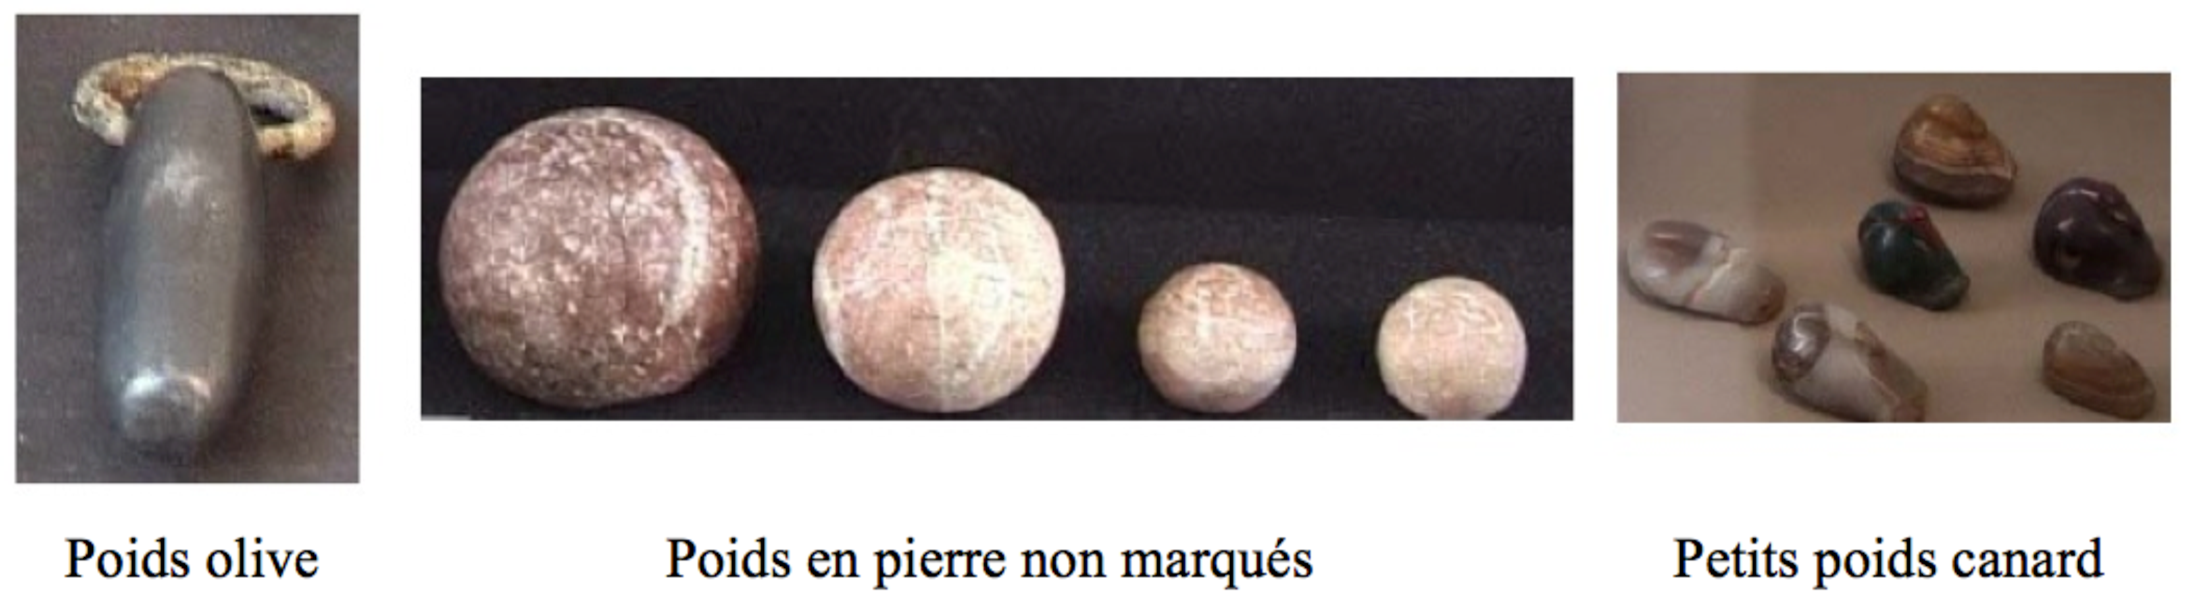
\includegraphics[width=15cm]{assets/figures/poids.pdf}
   \caption{Diverses références de masse utilisées durant l'Antiquité (Mésopotamie, Chine).}
   \label{fig:1.1}
\end{figure}
Les plus vieux poids (figure \ref{fig:1.1}) retrouvés en Mésopotamie sont en pierre polie.  Les fouilles des différents trésors montrent une caractéristique surprenante: l'anonymat des poids et celle des monnaies.  Ce fait ne démontre-t-il pas de solides relations de confiance entre les hommes et entre les groupes ?

Un autre constat surprenant: certains concepts de base de la métrologie mésopotamienne régissent l'infrastructure métrologique actuelle. Outre le fait que nous calculons, comme le faisaient les anciens habitants de la Mésopotamie, l'heure, les minutes, les secondes et les angles sur la même base sexagésimale, il semble encore nécessaire pour avoir confiance dans les échanges, de se mettre d'accord sur un étalon et la manière de s'en servir et donc de partager une culture métrologique commune au sein d'un " espace métrologique " commun.

\section{La référence commune : l'étalon}

Les anciens étalons sont gardés précieusement dans de hauts lieux symboliques.  Les poids mésopotamiens sont retrouvés dans d'anciens temples et palais.  à Athènes, une compagnie de quinze officiers prend soin des mesures originales et de l'inspection de l'étalonnage.  Chez les Romains, les étalons sont conservés au Capitole, dans le temple de Jupiter. Charlemagne les conserve dans son palais.  En Europe chrétienne, ils sont scellés sur les halles de marché et sur les murs extérieurs des églises.  Aujourd'hui encore, et ce pour un temps seulement, l'étalon de masse, dernier étalon matériel, est gardé précieusement sous trois cloches au Bureau international des Poids et mesures.

La référence commune, l'étalon, base de toute négociation réciproque et juste, a nécessité de tout temps un arbitrage entre plusieurs groupes de pression, marchands, acheteurs, paysans, classes dirigeantes, seigneurs fieffés, abbayes, pouvoir royal régulièrement, les marchands et la classe dirigeante cherchent, sous des formes diverses et renouvelées, à modifier les étalons pour servir leurs intérêts, ce qui va souvent de pair avec l'ignorance d'une part de la population des choses de la métrologie.

En contrepartie, à travers le temps, un phénomène tout aussi régulier apparaît, celui d'une tentative d'unification qui s'accompagne naturellement d'actions éducatives.  Des tablettes montrent que des écoles transmettent le savoir et les usages métrologiques en Mésopotamie et en Égypte.  Charlemagne unifie les mesures et développe le système scolaire.  À la Révolution française, la commission du mètre est confiée au Comité d'Instruction publique.

\section{Diversité des mesures}

Depuis l'Antiquité, ce ne sont pas sept unités fondamentales du système international, mais des milliers de mesures différentes, réinventées ou reconfigurées siècle après siècle qui vivent et s'atteignent. Tillet et Abeille présentent les " Observations de la Société Royale d'Agriculture sur l'Uniformité des Poids et mesures " réalisées par Villeneuve, à l'Assemblée nationale le 6 février 1790.

Ils constatent: " C'est un fait notoire que non seulement on se sert en France de quantité de poids différents qui portent tous le nom de livre, mais encore une multitude de boisseaux, d'aunes, de verges, de cannes, de toises, de pintes ; et que ces mesures diffèrent entre elles, quoiqu'on les désigne par le même nom ; que ces différences sont très considérables, non pas d'une province à une autre, ou d'une ville à une autre, mais dans la même ville, dans le même bourg, dans le même village. "

Les révolutionnaires ne sont pas les premiers à percevoir les inconvénients du foisonnement métrologique.  En France, les tentatives pour y remédier commencent avant l'an mille.  En 744, Childéric III voulut unifier les mesures.  Les capitulaires de Charlemagne en 789, 803 et 806 ordonnent que les mesures soient égales et les poids justes.: \textit{Aequales mensuras et rectas, pondera justa}.

Enfin, la métrologie est nommée en 1780 par Paucton dans son ouvrage métrologie ou traité des Mesures, Poids et Monnaies des anciens peuples et des Modernes.  Dans les Cahiers de doléances, les trois ordres demandent en substance et pour des raisons diverses qu'il n'y ait plus en France " qu'un roi, une loi, un poids et une mesure ".

La métrologie est alors confiée aux savants. Ceux-ci sont aussi philosophes, hommes de sciences et acteurs politiques de l'époque.  Le premier système cohérent de métrologie, le système métrique décimal est considéré comme un triomphe de l'esprit humain.  Il sera le vecteur d'une égalité entre les citoyens, de fraternité entre les peuples et celui de la libération des hommes.  Cette transformation de tous les repères subjectifs et sociaux est largement plébiscitée.

Petit, par exemple, écrit en 1809: " Aujourd'hui les poids et les mesures étant partout les mêmes, les affaires peuvent se traiter sans embarras, et il n'y a plus de nouveaux calculs à faire pour vendre ou pour acheter, quand on sait de quoi il s'agit ici. Il y a un temps qu'on désirait un pareil changement; l'intérêt public autant que les intérêts particuliers le sollicitaient : le nouveau système des poids et des mesures est donc, sous ce rapport, un bienfait incontestable ".

La métrologie, dorénavant confiée aux scientifiques et aux ingénieurs, va subir des transformations scientifiques, techniques et organisationnelles de très grande ampleur. Maintenant, avec le développement technique que nous connaissons, la métrologie du quotidien charpente et coordonne nos actes journaliers.  Le bon fonctionnement de nos infrastructures urbaines, la localisation par satellites, les normes alimentaires, les diagnostics médicaux, les règles d'échanges de biens internationaux, notre montre-bracelet ou le thermomètre familial, reposent sur une organisation internationale de la métrologie.

\section{Une culture métrologique commune}

Je vais régulièrement au salon de l'éducation qui a lieu annuellement à Paris. J'y effectue un sondage (\textit{c'est toujours Mme Cotteret qui s'exprime ici}). Nous ne pouvons pas parler d'échantillon statistiquement élaboré, mais d'un coup de loupe localement située.  En 2001, sur 91 personnes interrogées, élèves et adultes, 88 \% ne savent pas ce qu'est la métrologie.  En réponse à un QCM, 46 \% pensent que c'est la science des transports urbains ! En 2004, sur 131 personnes, 93 \% ne savent pas ce qu'est la métrologie. En réponse au QCM, 26 \% d'entre elles pensent que c'est la science de la prévision du temps.

En 2005, 50 enseignants sont sollicités pour répondre à la question : aujourd'hui, quelle est l'unité fondamentale de temps ?   50 \% répondent injustement, l'heure.  10 \% ne savent pas.  15 \% pensent que c'est la minute.  Seuls 25 \% énoncent la seconde !

Ces résultats font sourire... à moins qu'ils nous incitent à prendre conscience, comme le remarque Lord Kelvin (1824-1907), " ... qu'un changement de système de mesure n'est pas sans conséquence sur les systèmes de pensée.  À moins que ce ne soit l'évolution des idées qui conduise à bouleverser les unités de mesure ".

Alors que la technique et la science du début du XXIe siècle mobilisent des performances métrologiques jamais atteintes, pour la fabrication des microprocesseurs ou le positionnement par satellite par exemple, l'enseignement de la métrologie semble avoir décliné depuis un siècle. On peut aujourd'hui arriver jusqu'à un diplôme d'enseignement supérieur sans avoir pratiqué la mesure et ses calculs d'incertitude, donc vulnérable aux désinformations et aux erreurs de toutes natures.

Entre l'ignorance généralisée de culture métrologique des gens et une demande accrue d'une  opinion publique concernant des sujets hautement scientifiques et techniques, n'y a-t-il pas comme un déséquilibre ?  Jusqu'oé a-t-on oublié qu'une des bases de l'exercice du bon sens et de la citoyenneté passerait par une connaissance des systèmes de mesure qui gère notre société ?

La métrologie, ou science de la mesure, est considérée par les scientifiques comme le langage universel des sciences et des techniques.  Le système international a remplacé le système métrique décimal, mais qu'en est-il de sa diffusion ?  Qu'en est-il de la prise en compte par le plus grand nombre des grands changements tant paradigmatiques que cognitifs, symboliques et philosophiques que ce nouveau système de mesure transporte ?  Le dernier étalon matériel, le kilogramme sera prochainement considéré comme une pièce de musée et remplacé par une définition aussi obscure pour le public non averti que les définitions des autres unités de base.

" Jusqu'oé peut-on tromper le peuple ? " demandait Voltaire en 1756.  Peut-on comprendre les règles sans avoir accès aux règles qui font les règles ?  Sans culture métrologique appropriée, les décisions prises par des citoyens ignorants ne peuvent être que des opinions et, les opinions chacun le sait, sont manipulables.

En 1981, le Centre de Recherche sur la Culture Technique (CRCT) dans son Manifeste pour le développement de la culture technique constate : " La technique contemporaine n'est plus la technique des sociétés traditionnelles. Elle soutient par rapport à la recherche, un rapport tout différent. Technique et Science sont beaucoup plus proches l'une de l'autre que jadis, au point où l'ensemble scientifico-technique semble même constituer, pour le corps social, une menace globale qu'il lui est difficile à contrôler tant il lui est étranger. Il est ajouté: " Nous constatons que le milieu dans lequel nous vivons est de plus en plus constitué d'objets techniques inscrits dans une longue tradition historique, scientifique et culturelle.  Il semble donc évident que celui qui manque de culture technique vit dans l'ignorance de son propre milieu. "

\rm

\section{La mesure d'une grandeur physique}

On appelle \textbf{grandeur physique} toute propriété de la nature qui peut être quantifiée par la mesure ou le calcul, et dont les différentes valeurs possibles s'expriment à l'aide d'un nombre généralement accompagné d'une unité de mesure. Toute grandeur physique est en principe observable, et le terme d'\textbf{observable} est parfois utilisé pour désigner une grandeur physique que l'on mesure.

Par exemple, la masse et la longueur sont des grandeurs qui s'expriment respectivement en kilogramme et en mètres (ou en multiples de ces unités de base), alors que l'indice de réfraction d'un milieu s'exprime à l'aide d'un nombre sans unité et constitue une grandeur sans dimension.

L'addition et la soustraction de nombres ne sont possibles que s'ils sont relatifs à la même grandeur. En revanche, il est possible de multiplier ou de diviser des grandeurs différentes, auquel cas on obtient une nouvelle grandeur dérivée des deux autres. Par exemple, la vitesse est issue de la division de la longueur par le temps. Il existe donc théoriquement une infinité d'unités, mais seul un certain nombre d'entre elles sont utilisées dans la pratique.

On écrira le résultat de la mesure d'une grandeur sous la forme:
$$
X = \{X\}\ [X]
$$
où $X$ est le nom de la grandeur physique, $\{X\}$ est sa valeur numérique, et $[X]$ représente l'unité. \textbf{Toute grandeur physique est invariante, c'est-à-dire qu'elle ne dépend pas de l'unité dans laquelle on l'exprime}. Par exemple :
\begin{table}[htbp]
\begin{flushleft}
\begin{tabular}{lcll}
Longueur d'une règle & = & 30.48 & cm\\
& & 0.3048 & m\\
& & 12 & pouces\\
& & $1.646\times10^{-4}$ & mille marin.
\end{tabular}
\end{flushleft}
\end{table}

\begin{center}
\fbox{\begin{minipage}{12cm}\textbf{On voit ici que la valeur numérique dépend de l'unité choisie. En conséquence, celle-ci doit toujours être précisée !}\end{minipage}}
\end{center}